Una masa \(M=2\) está unida mediante un resorte \(k=2\) y un amortiguador viscoso \(c=5\), en paralelo, a una base móvil. Las cantidades se expresan en un sistema coherente de unidades. Tanto la posición de la masa x(t) como la de la base e(t) se miden hacia arriba desde el equilibrio inicial. La base sigue \(e(t)=10\sin(2\pi t)\), t>0; inicialmente la masa está en equilibrio y reposo. Halla x(t).

\Needspace{8.55cm}
\begin{center}
\begin{minipage}{\linewidth}
\centering
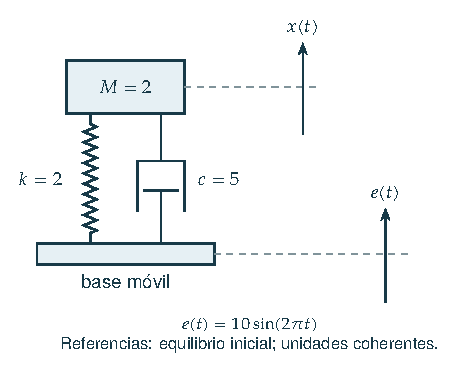
\includegraphics[width=8.7cm]{assets/M2-E0118-setup.pdf}\par
\smallskip{\small Masa y base móvil unidas mediante muelle y amortiguador en paralelo.\par}
\end{minipage}
\end{center}
